% Load essential packages
\usepackage{booktabs}
\usepackage{amsthm}
\usepackage{svg}
\usepackage[english]{babel}
\usepackage{longtable}
\usepackage{array}
\usepackage{multirow}
\usepackage{wrapfig}
\usepackage{colortbl}
\usepackage{pdflscape}
\usepackage{tabu}
\usepackage{threeparttable}
\usepackage{threeparttablex}
\usepackage[normalem]{ulem}
\usepackage{makecell}
\usepackage{xcolor}
\usepackage{hyperref}

% Figure title above figures
\usepackage{floatrow}
\floatsetup[figure]{capposition=top}

% Customize captions
\usepackage{caption}
\captionsetup[figure]{name=Figur, labelfont=bf, textfont=it, font=small}
\captionsetup[table]{name=Tabel, labelfont=bf, textfont=it, font=small}

% Customize chapter titles
\usepackage{titlesec}
\titleformat{\chapter}[display]
  {\normalfont\Huge\bfseries} % Formatting for the chapter block
  {\Large\bfseries Kapitel \thechapter} % Small size for "Kapitel" and bold for consistency
  {0pt} % Space between "Kapitel X" and the title
  {\Huge} % Larger size for the title
  [\vspace{-10pt}] % Adjust vertical spacing
\titlespacing*{\chapter}{0pt}{0pt}{10pt}


% Rename table of contents and appendix
\addto\captionsenglish{\renewcommand{\contentsname}{Indholdsfortegnelse}}
\addto\captionsenglish{\renewcommand{\appendixname}{Bilag}}

% Page layout
\usepackage[a4paper, top=1in, bottom=1in, left=1.5in, right=1in, bindingoffset=0.5in]{geometry}

% Custom spacing for theorem environments
\makeatletter
\def\thm@space@setup{
  \thm@preskip=8pt plus 2pt minus 4pt
  \thm@postskip=\thm@preskip
}
\makeatother

% Title page with image
\usepackage{titling}
\pretitle{\begin{center}
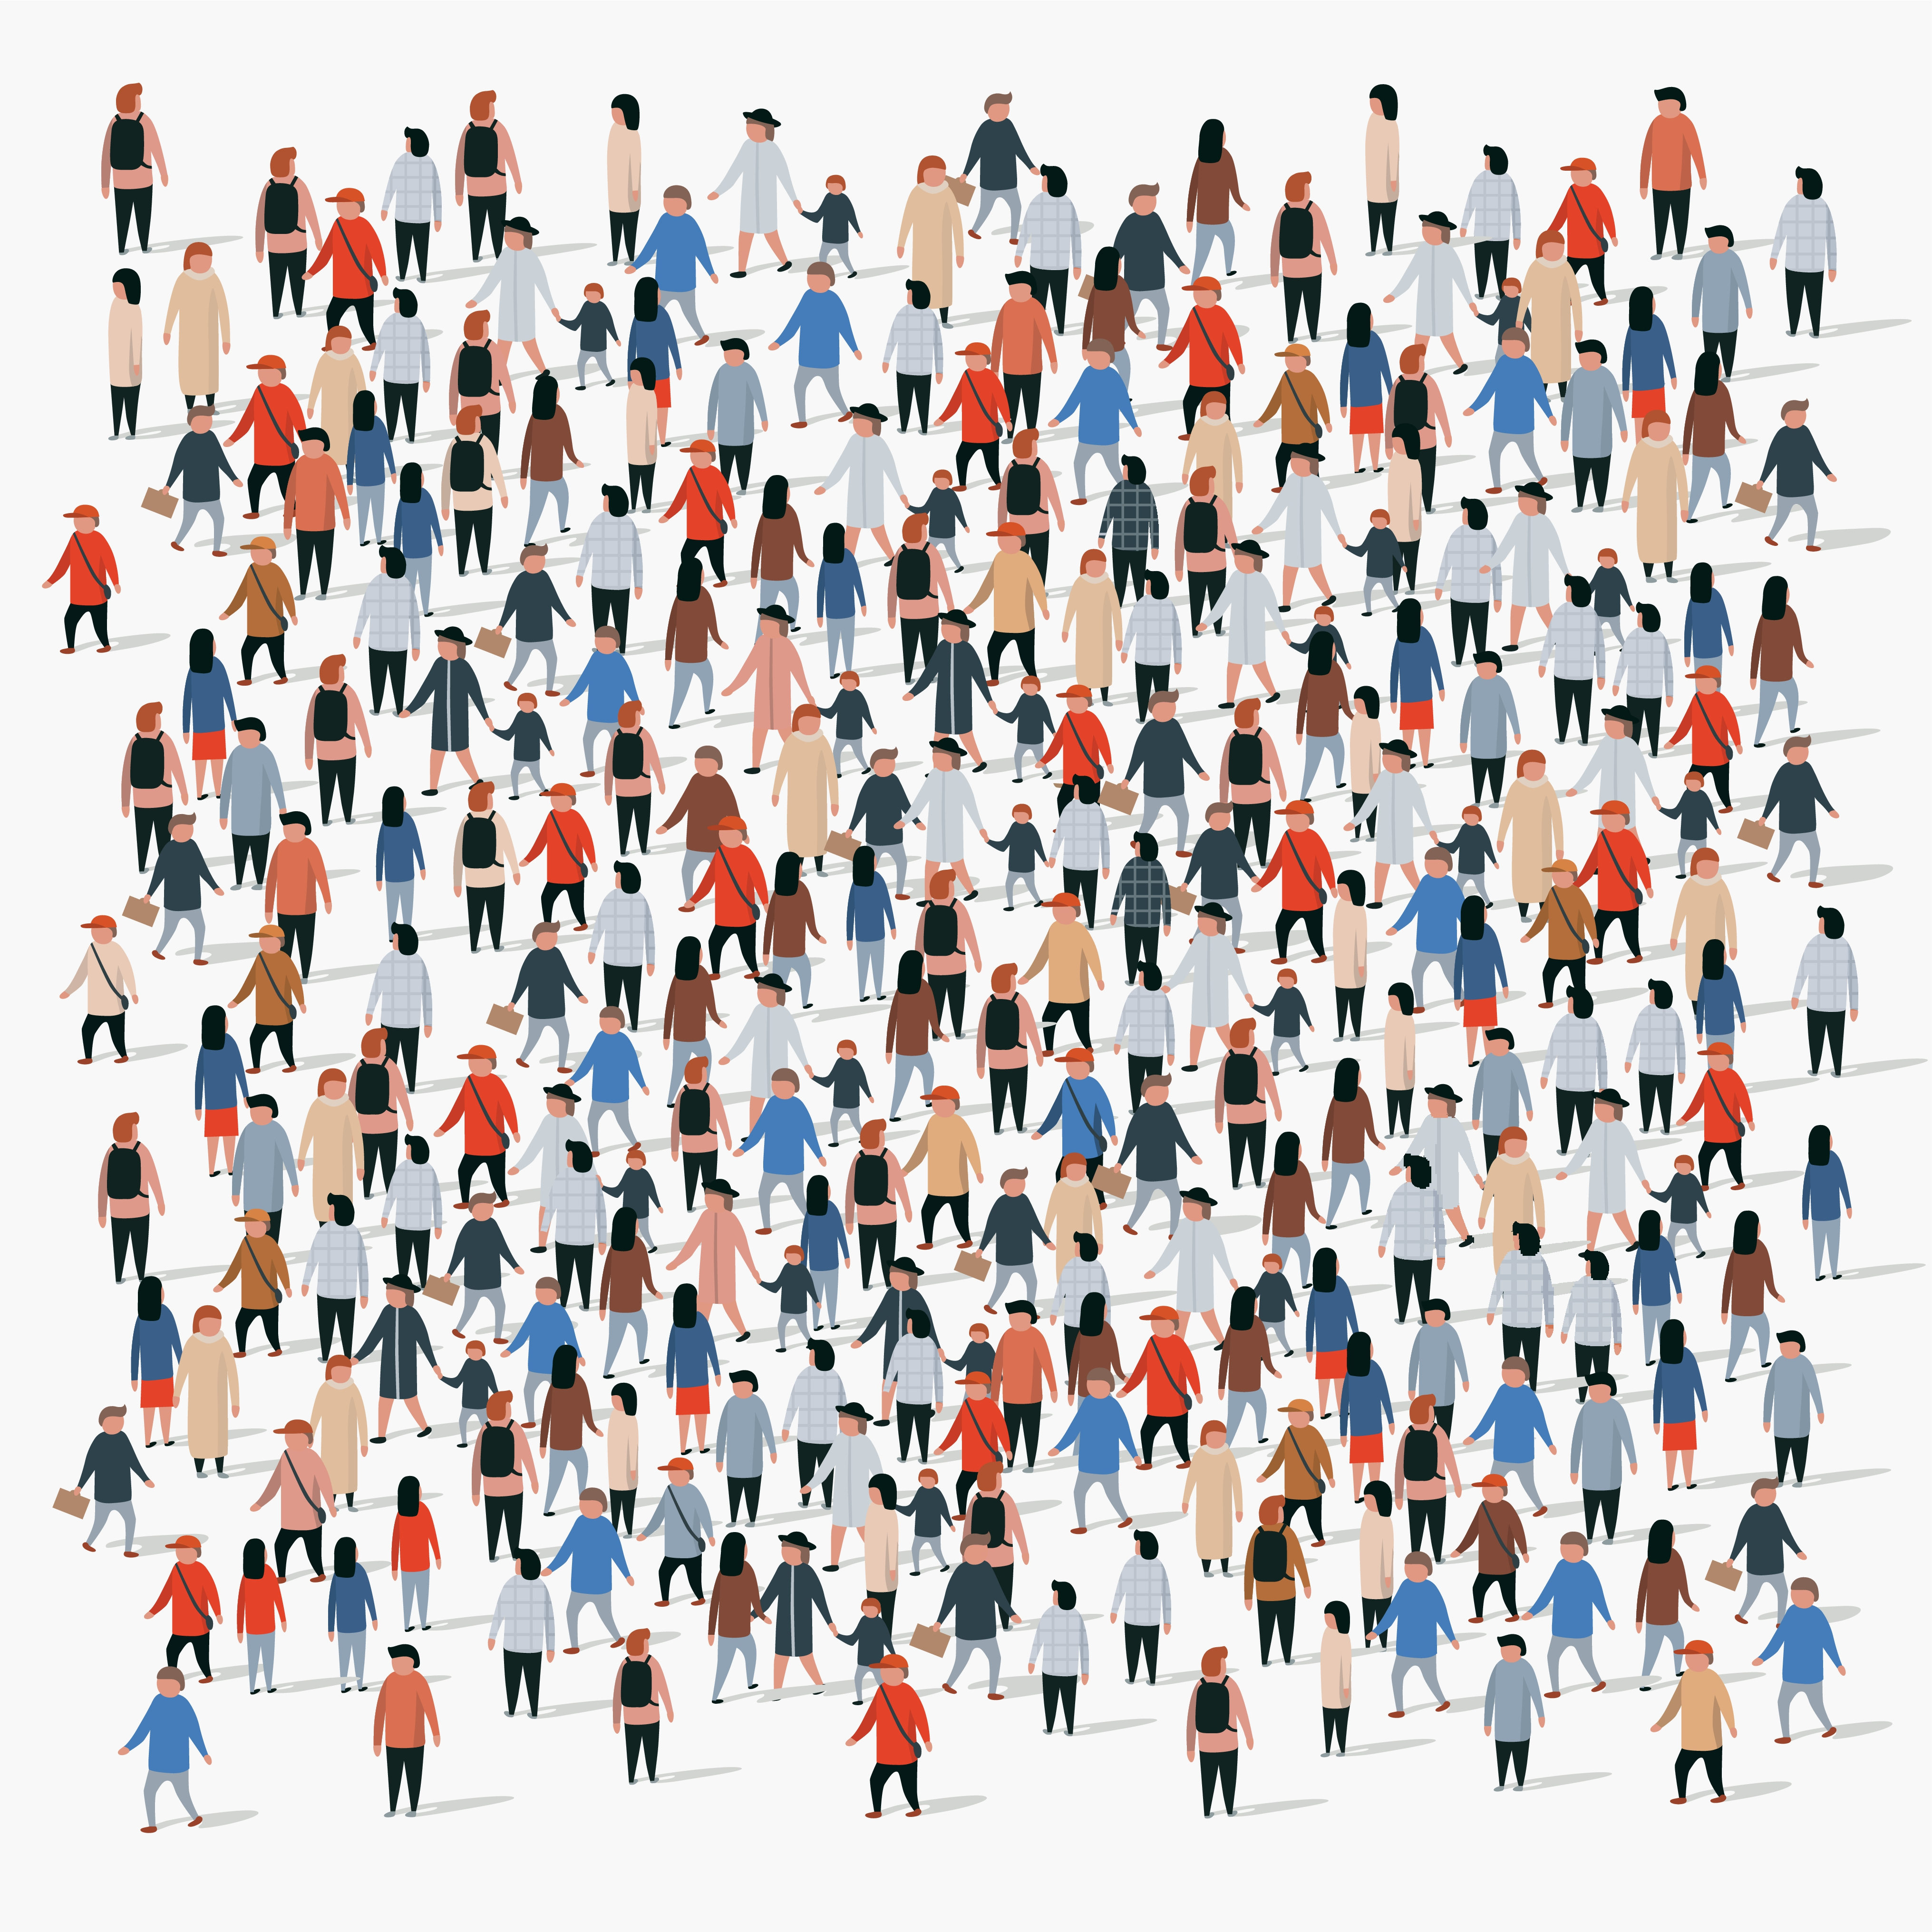
\includegraphics[width=5in,height=5in]{images/kap1.jpg}\LARGE\\}
\posttitle{\end{center}}

% Font setup
\usepackage{fontspec}
\setmainfont[
    BoldFont={Fira Sans SemiBold},
    ItalicFont={Fira Sans Italic},
    BoldItalicFont={Fira Sans SemiBold Italic}
]{Fira Sans}

% Page format
\usepackage{fancyhdr}
\pagestyle{fancy}

\renewcommand{\chaptermark}[1]{\markboth{#1}{}}

\fancyhead[L]{\footnotesize Kapitel \thechapter: \leftmark}
\fancyhead[R]{\footnotesize \thepage} % Page number

% Roman page numbering before chapter 1
\pagenumbering{gobble}
